%\documentclass[sigplan]{acmart}
\documentclass[sigplan]{acmart}

\usepackage[latin9]{inputenc}
\usepackage{booktabs} % For formal tables

% To include figures
\usepackage{graphicx}

% For TiKZ plots
\usepackage{tikz,pgfplots}

% To typeset SYCL programs
\usepackage{sycl}

% URL looks nicer in Teletype style
\urlstyle{tt}

% An alternative is
% https://tex.stackexchange.com/questions/266401/frame-a-line-in-an-environnement-lstlisting
% https://tex.stackexchange.com/questions/8851/how-can-i-highlight-some-lines-from-source-code
% /usr/share/doc/texlive-doc/latex/tikzmark/tikzmark.pdf
\usetikzlibrary{tikzmark}
\usetikzmarklibrary{listings}
\usepackage{balloon_rk_no_beamer}

% I got often this error:
% pdfTeX error (ext4): \pdfendlink ended up in different nesting level than \pdfstartlink.
%
% https://github.com/ho-tex/hyperref/issues/19
% https://www.overleaf.com/help/246-what-does-slash-pdfendlink-ended-up-in-different-nesting-level-than-slash-pdfstartlink-mean
%
% To remove the hyperlink output to look in the PDF where a link is broken
% on different columns:
%\hypersetup{draft}

% Copyright
%\setcopyright{none}
%\setcopyright{acmcopyright}
\setcopyright{acmlicensed}
%\setcopyright{rightsretained}
%\setcopyright{usgov}
%\setcopyright{usgovmixed}
%\setcopyright{cagov}
%\setcopyright{cagovmixed}

% pgfplot settings
\pgfplotsset{compat=newest}

\pgfplotsset{
    % #1: index in the group(0,1,2,...)
    % #2: number of plots of that group
    bar group size/.style 2 args={
        /pgf/bar shift={%
                % total width = n*w + (n-1)*skip
                % -> subtract half for centering
                -0.5*(#2*\pgfplotbarwidth +
                (#2-1)* \pgfkeysvalueof{/pgfplots/bar group skip})  +
                % the '0.5*w' is for centering
                (.5+#1)*\pgfplotbarwidth +
                #1*\pgfkeysvalueof{/pgfplots/bar group skip}},%
    },
    bar group skip/.initial=2pt,
    plot 0/.style={black,fill=blue!90!white,mark=none},%
    plot 1/.style={black,fill=blue!30!white,mark=none},%
    plot 2/.style={black,fill=green!90!white,mark=none},%
    plot 3/.style={black,fill=green!30!white,mark=none},%
    plot 4/.style={black,fill=purple!90!white,mark=none},%
    plot 5/.style={black,fill=red!90!white,mark=none},%
}

% DOI
\acmDOI{10.1145/3204919.3204937}

% ISBN
\acmISBN{978-1-4503-6439-3/18/05}

%Conference
\acmConference[IWOCL '18]{International Workshop on OpenCL (IWOCL '18)}{May 14--16, 2018}{Oxford, United Kingdom}
\acmBooktitle{IWOCL '18: International Workshop on OpenCL (IWOCL '18), May 14--16, 2018, Oxford, United Kingdom}

\acmMonth{5}
\acmYear{2018}
\copyrightyear{2018}
\acmPrice{15.00}

%\acmBadgeL[http://ctuning.org/ae/ppopp2016.html]{ae-logo}
%\acmBadgeR[http://ctuning.org/ae/ppopp2016.html]{ae-logo}

\sloppy
\begin{document}

\title{Early experiments using SYCL single-source modern C++ on Xilinx FPGA}
\subtitle{Extended Abstract of Technical Presentation}

\author{Ronan Keryell}
\email{rkeryell@xilinx.com}

\author{Lin-Ya Yu}
\email{linyay@xilinx.com}

\affiliation{%
  \institution{Xilinx Research Labs}
  \streetaddress{2020 Bianconi Avenue}
  \city{Dublin}
  \country{Ireland}
  \postcode{D24 T683}
}


\begin{abstract}
  Heterogeneous computing is required in systems ranging from low-end
  embedded systems up to the high-end HPC systems to reach
  high-performance while keeping power consumption low. Having more
  and more CPU and accelerators such as FPGA creates challenges for
  the programmer, requiring even more expertise of them. Fortunately,
  new modern C++-based domain-specific languages, such as the SYCL
  open standard from Khronos Group, simplify the programming at the
  full system level while keeping high performance.

  SYCL is a single-source programming model providing a task graph of
  heterogeneous kernels that can be run on various accelerators or
  even just the CPU. The memory heterogeneity is abstracted through
  buffer objects and the memory usage is abstracted with accessor
  objects. From these accessors, the task graph is implicitly
  constructed, the synchronizations and the data movements across the
  various physical memories are done automatically, by opposition to
  OpenCL or CUDA.

  triSYCL is an on-going open-source project used to experiment with
  the SYCL standard, based on C++17, OpenCL, OpenMP and Clang/LLVM.
  We have extended this framework to target Xilinx SDx tool to compile
  some SYCL programs to run on a CPU host connected to some FPGA PCIe
  cards, by using OpenCL and SPIR standards from Khronos.

  While SYCL provides functional portability, we made a few
  FPGA-friendly extensions to express some optimization to the SDx
  back-end in a pure C++ way.

  We present some interesting preliminary results with simple
  benchmarks showing how to express pipeline, dataflow and
  array-partitioning and we compare with the implementation written
  using other languages available for Xilinx FPGA: HLS C++ and OpenCL
  C.

  %We end up with an experiment using the current CNL proposal for
  %fixed-point data types in ISO C++, giving guidance to the ISO
  %committee and demonstrating the advantage of pure standard C++ for
  %all-programmable devices beyond CPU, such as FPGA MPSoC.
\end{abstract}

%
% The code below should be generated by the tool at
% http://dl.acm.org/ccs.cfm
\begin{CCSXML}
<ccs2012>
<concept>
<concept_id>10010147.10010169.10010175</concept_id>
<concept_desc>Computing methodologies~Parallel programming languages</concept_desc>
<concept_significance>500</concept_significance>
</concept>
<concept>
<concept_id>10010147.10010169.10010170.10010174</concept_id>
<concept_desc>Computing methodologies~Massively parallel algorithms</concept_desc>
<concept_significance>300</concept_significance>
</concept>
<concept>
<concept_id>10011007.10011006.10011008.10011009.10010175</concept_id>
<concept_desc>Software and its engineering~Parallel programming languages</concept_desc>
<concept_significance>500</concept_significance>
</concept>
<concept>
<concept_id>10011007.10011006.10011050.10011017</concept_id>
<concept_desc>Software and its engineering~Domain specific languages</concept_desc>
<concept_significance>500</concept_significance>
</concept>
<concept>
<concept_id>10011007.10011006.10011066.10011067</concept_id>
<concept_desc>Software and its engineering~Object oriented frameworks</concept_desc>
<concept_significance>300</concept_significance>
</concept>
<concept>
<concept_id>10010520.10010521.10010542.10010546</concept_id>
<concept_desc>Computer systems organization~Heterogeneous (hybrid) systems</concept_desc>
<concept_significance>300</concept_significance>
</concept>
</ccs2012>
\end{CCSXML}

\ccsdesc[500]{Computing methodologies~Parallel programming languages}
\ccsdesc[300]{Computing methodologies~Massively parallel algorithms}
\ccsdesc[500]{Software and its engineering~Parallel programming languages}
\ccsdesc[500]{Software and its engineering~Domain specific languages}
\ccsdesc[300]{Software and its engineering~Object oriented frameworks}
\ccsdesc[300]{Computer systems organization~Heterogeneous (hybrid) systems}
% We no longer use \terms command
%\terms{Theory}

\keywords{SYCL, C++17, DSeL, FPGA, reconfigurable computing, OpenCL,
  SPIR, Clang, LLVM, triSYCL}


\maketitle

\section{Introduction}
\label{sec:introduction}

Computing architectures nowadays are huge hybrid multi-processor
system-on-chips with different kinds of processors, GPU, configurable
specific accelerators (video CODEC...), reconfigurable programmable
logic (FPGA), various hierarchies of memory and memory interfaces,
configurable IO and network support, security support, and power control
etc. High-performance applications may use a hierarchy of such systems
scaling up towards utilizing a full-scale data-center.

So the programmer is facing a fractal architecture, demanding
also more and more control for power efficiency. This tends to require
a dense fractal set of skills and tools.

SYCL \cite{SYCL-1.2.1,SYCL-2.2-provisional} is a new open standard
from Khronos Group aiming at solving some of the programming issues
related to heterogeneous computing.  This pure C++14 (for SYCL 1.2.1)
or C++17 (for SYCL 2.2) domain-specific embedded language allows the
programmer to write single-source C++ host code with accelerated code
expressed as functors. The data accesses are described with accessor
objects that implicitly define a task graph that can be asynchronously
scheduled on a distributed-memory system including several CPU and
accelerators.

This programming model is quite generic but provides also an
interoperability mode with the OpenCL realm, another standard from
Khronos Group aimed at heterogeneous computing with a C host API and
separate language for the kernels (C, C++, SPIR and SPIR-V).  This
allows a SYCL C++ application to recycle existing OpenCL kernels into
a higher level C++ programming model, relieving the programmer from
explicitly defining the memory transfers.

In this article we present in Section~\ref{sec:sycl} the SYCL standard,
then in Section~\ref{sec:fine-grain-parallel} how to express pipelined and
dataflow execution in SYCL and how dealing with partitioned arrays in
Section~\ref{sec:array-partitioning}.


\section{SYCL}
\label{sec:sycl}

\begin{figure*}
  \balloono{comment}{example}{17}{26}
  \balloon{comment}{example}{22}{25}
  \balloono{comment}{example}{28}{37}
  \balloon{comment}{example}{33}{36}
  \balloono{comment}{example}{39}{50}
  \balloon{comment}{example}{46}{49}
  
\begin{tikzpicture}[remember picture,overlay]
    \draw [overlay,->,very thick,red] (pic cs:PA) to[bend left] (pic cs:CA);
    \draw [overlay,->,very thick,red] (pic cs:PB) to[bend left] (pic cs:CB);
    \draw [overlay,->,very thick,red] (pic cs:PC) to[bend right] (pic cs:CC);
  \end{tikzpicture}
  \begin{tabular}{c}
    \begin{lstlisting}[basicstyle=\scriptsize,name=example]
// Demonstrate the use of an asynchronous task graph of kernels to initialize and add 2 matrices.
#include <CL/sycl.hpp>
#include <iostream>
using namespace cl::sycl;
// Size of the matrices
constexpr size_t N = 2000;
constexpr size_t M = 3000;

int main() {
  // Create a queue to work on
  queue q;
  // Create some 2D buffers of N*M floats for our matrices
  buffer<float, 2> a { { N, M } };
  buffer<float, 2> b { { N, M } };
  buffer<float, 2> c { { N, M } };
  // Launch a first asynchronous kernel to initialize a
  q.submit([&] (handler &cgh) {
      // The kernel writes a, so get a write accessor on it
      auto A = a.get_access<access::mode::write>(cgh);�\tikzmark{PA}�

      // Enqueue a parallel kernel iterating on a N*M 2D iteration space
      cgh.parallel_for<class init_a>({ N, M },
                                     [=] (id<2> index) {
                                       A[index] = index[0]*2 + index[1];
                                     });
    });
  // Launch an asynchronous kernel to initialize b
  q.submit([&] (handler &cgh) {
      // The kernel writes b, so get a write accessor on it
      auto B = b.get_access<access::mode::write>(cgh);�\tikzmark{PB}�
      /* From the access pattern above, the SYCL runtime detects this command group is independent from the first one and can be scheduled independently.
         Enqueue a parallel kernel iterating on a N*M 2D iteration space */
      cgh.parallel_for<class init_b>({ N, M },
                                     [=] (id<2> index) {
                                       B[index] = index[0]*2014 + index[1]*42;
                                     });
    });
  // Launch an asynchronous kernel to compute matrix addition c = a + b
    q.submit([&] (handler &cgh) {
        // In the kernel a and b are read, but c is written
        auto A = a.get_access<access::mode::read>(cgh);�\tikzmark{CA}�
        auto B = b.get_access<access::mode::read>(cgh);�\tikzmark{CB}�
        auto C = �\tikzmark{PC}�c.get_access<access::mode::write>(cgh);
        // From these accessors, the SYCL runtime will ensure that when this kernel is run, the kernels computing
        // a and b completed. Then Enqueue a parallel kernel iterating on a N*M 2D iteration space
        cgh.parallel_for<class matrix_add>({ N, M },
                                           [=] (id<2> index) {
                                             C[index] = A[index] + B[index];
                                           });
      });
    /* Request an accessor to read c from the host-side. The SYCL runtime ensures that c is ready when the accessor is returned */
    auto C = �\tikzmark{CC}�c.get_access<access::mode::read>();
    std::cout << std::endl << "Result:" << std::endl;
    for (size_t i = 0; i < N; i++)
      for (size_t j = 0; j < M; j++)
        // Compare the result to the analytic value
        if (C[i][j] != i*(2 + 2014) + j*(1 + 42)) {
          std::cout << "Wrong value " << C[i][j] << " on element "
                    << i << ' ' << j << std::endl;
          exit(-1);
        }
  std::cout << "Accurate computation!" << std::endl;
  return 0;
}
    \end{lstlisting}
  \end{tabular}
  \caption{Example of a SYCL C++ program producing and adding 2
    matrices, coming from
    \url{https://github.com/triSYCL/triSYCL/blob/master/tests/examples/demo_parallel_matrix_add.cpp}.\label{fig:SYCL-example}}
\end{figure*}

SYCL \cite{SYCL-1.2.1,SYCL-2.2-provisional} (pronounced ``sickle'') is a
royalty-free, cross-platform abstraction C++ programming model for
OpenCL \cite{OpenCL-API-2.2-provisional,
  OpenCL-C++-2.2-provisional}. SYCL builds on the underlying concepts,
portability and efficiency of OpenCL while adding much of the ease of
use and flexibility of single-source C++.

Developers using SYCL are able to write standard C++14/C++17 code,
with many of the techniques they are accustomed to, such as
inheritance and templating. At the same time developers have access to
the full range of capabilities of OpenCL both through the features of
the SYCL libraries and, where necessary, through interoperation with
code written directly to the OpenCL
APIs~\cite{OpenCL-API-2.2-provisional}.

SYCL implements a single-source multiple compiler-passes design which
offers the power of source integration while allowing tool-chains to
remain flexible. This design supports embedding of code intended to be
compiled for an OpenCL device, for example a GPU or an FPGA, inline
with host code.

SYCL is a pure single-source C++ DSeL (Domain-Specific Embedded
Language) providing simpler abstractions for heterogeneous
computing. In Figure~\ref{fig:SYCL-example} is presented a small
application using SYCL concepts to create a graph of 3 asynchronous
tasks to initialize 2 matrices and addition them before checking for
the final result.

The main interesting features that SYCL brings are asynchronous task
graphs, hierarchical parallelism, buffers defining location-independent
storage, accessors to express usage for buffers and other objects,
implicit dependency graph, automatic data motion, automatic overlapping
kernels and communications, single-source, host fallback for debugging or
when no accelerator is available and cross-platform (buffers used by
different devices from different vendors), OpenCL interoperability mode.

SYCL retains the execution model, runtime feature set and device
capabilities of the underlying OpenCL standard. This is why SYCL
1.2.1~\cite{SYCL-1.2.1} targets devices with OpenCL
1.2~\cite{OpenCL-API+C-1.2} capabilities, while SYCL
2.2~\cite{SYCL-2.2-provisional} targets devices with OpenCL
2.2~\cite{OpenCL-API-2.2-provisional} capabilities, adding for example
the pipes and the shared virtual memory between the host and devices.

The OpenCL C specification imposes some limitations on the full range
of C++ features that SYCL is able to support. This ensures portability
of device code across as wide a range of devices as possible.

As a result, while the code can be written in standard C++ syntax with
interoperability with standard C++ programs, the entire set of C++
features is not available in SYCL device code. In particular, SYCL
device code, as defined by this specification, does not support
virtual function calls, function pointers in general, exceptions,
runtime type information or the full set of C++ libraries that may
depend on these features or on features of a particular host compiler.

Actually these features are anyway often used in C++ high-performance code
in the hot-path because of performance issues.  Fortunately, the use of
C++ features such as templates and inheritance on top of the OpenCL
execution model opens a wide scope for innovation in software design for
heterogeneous systems, giving workarounds for some of the unsupported
features.

Clean integration of device and host code within a single C++ type
system enables the development of modern, templated libraries that
build simple, yet efficient, interfaces to offer more developers
access to OpenCL capabilities and devices. SYCL is intended to serve
as a foundation for innovation in programming models for heterogeneous
systems, that builds on an open and widely implemented standard
foundation in the form of OpenCL.

This is why the OpenCL version of TensorFlow \cite{TensorFlow-1.0},
the C++ machine learning framework from Google, is actually using SYCL
instead of plain OpenCL.

SYCL is one of the candidates giving inputs on parallelism and
heterogeneous computing to the C++ ISO/IEC JTC1/SC22/WG21
standardization committee
\cite{C++:P00236R0:SYCL,C++:P0362R0,C++:P0363R0,C++:P0367R0}.
\iffalse
  WG21,
presented at C++ F2F committee Jacksonville 2016/02
% http://www.open-std.org/jtc1/sc22/wg21/docs/papers/2016/p0236r0.pdf
% https://groups.google.com/a/isocpp.org/forum/#!topic/sg14/8GWWDulGE7o
 Oulu 2016/06
% http://www.open-std.org/jtc1/sc22/wg21/docs/papers/2016/p0362r0.pdf
% http://www.open-std.org/jtc1/sc22/wg21/docs/papers/2016/p0363r0.pdf
% http://www.open-std.org/jtc1/sc22/wg21/docs/papers/2016/p0367r0.pdf
 Khronos committed to provide Open Source implementations of OpenCL and SYCL
\fi


\section{Fine grain parallel execution}
\label{sec:fine-grain-parallel}

High-level programs on FPGA are typically compiled with each operation
translated in some hardware implementation. Compared to the compilation
for architectures with fixed hardware functions such as CPU, DSP or GPU,
that means that the hardware implementations of the operations do coexist
in space inside the FPGA, which means that they can be used in parallel to
increase the throughput of the system.

In a ``normal'' computer this is not a parameter to be taken in
consideration, but for FPGA this is something useful to express somehow,
when compiling a C/C++ program for FPGA. Each FPGA vendor have some
extensions to express these optimizations, such as
\cite{IWOCL2016:OpenCL_Xilinx_FPGA,
  Xilinx:UG1207-2017.4:SDAccel_Profiling_Optimization,
  Xilinx:UG1235-2017.4:SDSoC_Profiling_Optimization,
  Xilinx:UG1270-2017.4:HLS_Optimization_Methodology,
  Xilinx:UG1253-2017.4:SDx_Pragma_Reference}, based on
\lstinline|#pragma|, attributes or even configuration files or compiler
options.

The issues  with extensions such  as \lstinline|#pragma| or  attributes is
that they require a specific compiler  to parse and understand them.  This
prevents some  emulation on  CPU for example,  with some  compile-time and
run-time checking.

In our SYCL implementation, we prefer to have some pure C++ function-based
and class-based extensions, compatible with CPU emulation and more aligned
with SYCL DSeL philosophy.


\subsection{Pipelined execution}
\label{sec:pipelined-execution}

\begin{figure}
  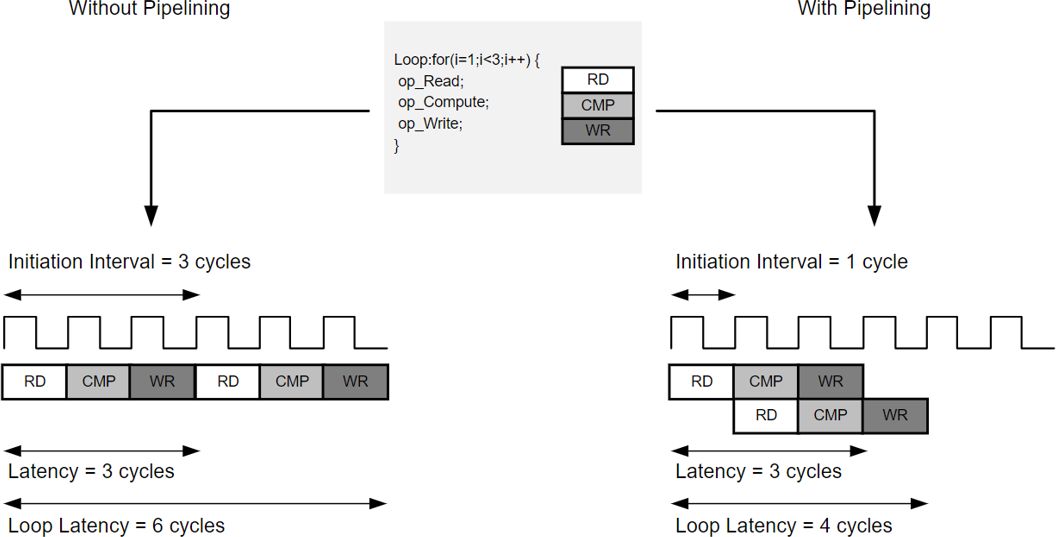
\includegraphics[width=\hsize]{Figures/pipeline_execution}
  \caption{Execution of operations of a loop in normal and pipelined way.}
  \label{fig:pipelined-execution}
\end{figure}

In a loop, all the operations of an iteration will be executed
sequentially, as shown on Figure~\ref{fig:pipelined-execution}. The
operations are used in sequence and if there is no intra-loop dependency
in the program preventing this, the operations from different iterations
can actually be executed in parallel, to increase the throughput using the
pipelined execution shown also on Figure~\ref{fig:pipelined-execution}, by
reducing the \emph{initiation interval}, to use the FPGA jargon.

\begin{figure}
  \balloon{comment}{PipelinedTriSYCL}{5}{5}
  \balloon{comment}{PipelinedTriSYCL}{9}{9}
  \begin{tabular}{c}
    \begin{lstlisting}[basicstyle=\scriptsize,name=PipelinedTriSYCL]
template<typename T, typename U>
void compute(T *buffer_in, U *buffer_out) {
  for(int i = 0; i < NUM_ROWS; ++i) {
    for (int j = 0; j < ELE_PER_ROW; ++j) {
      xilinx::pipeline([&] {
        int inTmp = buffer_in[ELE_PER_ROW*i+j];
        int outTmp = inTmp * ALPHA;
        buffer_out[ELE_PER_ROW*i+j] = outTmp;
      });
    }
  }
}
    \end{lstlisting}
  \end{tabular}
  \caption{Example of a typical loop with pipelined execution. What is
    added is shown with a blue background.}
  \label{fig:SYCL-pipelined}
\end{figure}

As shown on Figure~\ref{fig:SYCL-pipelined}, we chose to mark a zone to be
pipelined with a kind of decorator \emph{� la} Python
\cite{Python:PEP318:decorators} \lstinline|xilinx::pipeline(...)| taking a
functor, typically expressed in modern C++ as a lambda expression.


\subsection{Dataflow execution}
\label{sec:dataflow-execution}

While pipeline execution is very fine-grain parallelism, a coarser-grain
parallelism can be used when having different functions with data flowing
from one function to another: dataflow execution.

\begin{figure}
  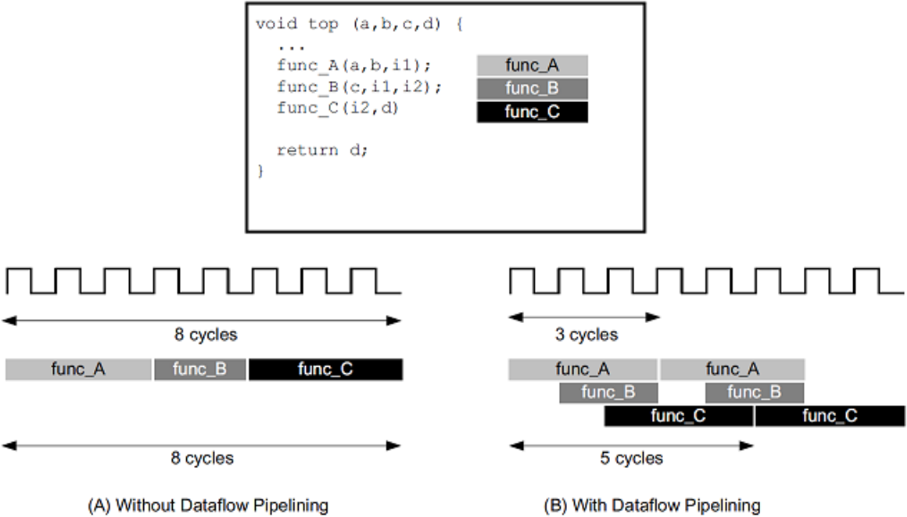
\includegraphics[width=\hsize]{Figures/dataflow_execution}
  \caption{Execution of functions without or with dataflow mode.}
  \label{fig:dataflow-execution}
\end{figure}

Since on the FPGA the functions are instantiated in hardware, they can
execute in parallel and if data dependencies allow it, data can move from
one function to another either using dual-buffering ping-pong buffers
(preventing the time-consuming and power-hungry external memory) or even a
FIFO (preventing the use of more complex power-hungry memory access), as
shown on Figure~\ref{fig:dataflow-execution}.

\begin{figure}
  \balloon{comment}{DataFlowTriSYCL}{5}{5}
  \balloon{comment}{DataFlowTriSYCL}{7}{7}
  \balloon{comment}{DataFlowTriSYCL}{14}{14}
  \balloon{comment}{DataFlowTriSYCL}{18}{18}
  \balloon{comment}{DataFlowTriSYCL}{25}{25}
  \balloon{comment}{DataFlowTriSYCL}{27}{27}
  \balloon{comment}{DataFlowTriSYCL}{27}{27}
  \balloono{comment}{DataFlowTriSYCL}{37}{37}
  \balloono{comment}{DataFlowTriSYCL}{41}{41}
  \begin{tabular}{c}
    \begin{lstlisting}[basicstyle=\scriptsize,name=DataFlowTriSYCL]
template<typename T, typename U>
void readInput(T *buffer_in, const U &d_b) {
 for(int i = 0; i < NUM_ROWS; ++i)
  for (int j = 0; j < ELE_PER_ROW; ++j)
    xilinx::pipeline([&] {
      buffer_in[ELE_PER_ROW*i+j] = d_b[ELE_PER_ROW*i+j];
    });
}

template<typename T, typename U>
void compute(T *buffer_in, U *buffer_out) {
 for(int i = 0; i < NUM_ROWS; ++i)
  for (int j = 0; j < ELE_PER_ROW; ++j)
    xilinx::pipeline([&] {
      int inTmp = buffer_in[ELE_PER_ROW*i+j];
      int outTmp = inTmp * ALPHA;
      buffer_out[ELE_PER_ROW*i+j] = outTmp;
    });
}

template<typename T, typename U>
void writeOutput(T *buffer_out, const U &d_a) {
 for(int i = 0; i < NUM_ROWS; ++i)
  for (int j = 0; j < ELE_PER_ROW; ++j)
    xilinx::pipeline([&] {
      d_a[ELE_PER_ROW*i+j] = buffer_out[ELE_PER_ROW*i+j];
    });
}

cgh.single_task<class add>
           ([=,
             d_a = drt::accessor<decltype(a_a)> { a_a },
             d_b = drt::accessor<decltype(a_b)> { a_b }
             ] {
                 int buffer_in[BLOCK_SIZE];
                 int buffer_out[BLOCK_SIZE];
                 xilinx::dataflow([&] {
                     readInput(buffer_in, d_b);
                     compute(buffer_in, buffer_out);
                     writeOutput(buffer_out, d_a);
                 });
               });
    \end{lstlisting}
  \end{tabular}
  \caption{Example of a typical loop with functional dataflow execution
    with also pipelined execution of each function. What is added for
    dataflow execution has an orange background and for a pipelined
    execution has a blue background.}
  \label{fig:SYCL-dataflow}
\end{figure}

To mark an area in the program to apply such an optimization, we use the
same trick as for pipelining (\S~\ref{sec:pipelined-execution}) with a
\lstinline|xilinx::dataflow(...)| as shown on
Figure~\ref{fig:SYCL-dataflow}. Currently we have a limitation in our
device compiler and runtime that requires changing the lambda captures
with \lstinline|drt::accessor| like adding in the example some lines such
as
\begin{lstlisting}[basicstyle=\scriptsize,name=DataFlowTriSYCL]
d_a = drt::accessor<decltype(a_a)> { a_a },
\end{lstlisting}
but this limitation should be removed soon.


\subsection{Experiments with pipelined and dataflow execution}
\label{sec:experiments-pipelined-dataflow}

We have run various experiments on a benchmark transferring 2D arrays with
and without these optimizations in SYCL (code from
Figure~\ref{fig:SYCL-dataflow}), but also with non-single source HLS C++
or OpenCL C kernels, coming from
\cite{Xilinx:GitHub:SDAccel_Examples}. The SYCL examples have been
translated for this study from the HLS C++ and OpenCL examples, leading to
quite shorter examples, typically less than 100 lines compared to the
original 250+ line examples in HLS C++ or OpenCL C.

\begin{figure}
  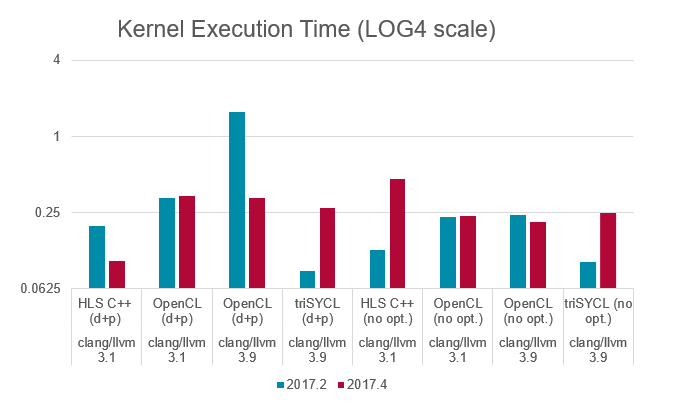
\includegraphics[width=\hsize]{Figures/dataflow_pipeline_kernel_exe_time}
  \caption{Comparison of execution times of 2D array transfers with
    various tools and languages with a Xilinx FPGA acceleration card.}
  \label{fig:2D-array-benchmark-comparison}
\end{figure}

When possible, we compared 2 different versions of the tools (Xilinx SDx
2017.2 and 2017.4) that can also be configured to use either a Clang/LLVM
3.1 or 3.9 front-end. The performance results are shown on
Figure~\ref{fig:2D-array-benchmark-comparison} for a default kernel
execution clock of 200~MHz with an ADM-PCIE-7V3 PCIe FPGA accelerator
card~\cite{ADM-PCIE-7V3} plugged into an Ubuntu 17.10 Linux system with an
Intel core i7-6700 CPU and 64~GB of RAM. The triSYCL device compiler is
using Clang/LLVM 3.9 and we used the Xilinx SDx OpenCL runtime 2017.2.

The performance of triSYCL are quite reasonable compared to some other
programming models and tools, and sometimes even gives the best
result. This shows that higher-level programming model does not mean
always trading programmability with execution efficiency, for example
because the single-source approach provides to the compiler a global
interprocedural view between host code and device code, allowing for
example some variable that appears to be a constant on the host-side to be
directly evaluated on the device code without requiring some explicit
host-device PCIe data transfer as for OpenCL or HLS C++.

We have not yet looked deeply at the understanding of the different
performance results and QoR (quality of results). The complexity comes
from comparing different tool versions, using different Clang/LLVM
versions, with different optimizing paths, and the various Xilinx tool
versions exercising different heuristics with different behaviour
according to the input languages (OpenCL, HLS C++ and SPIR-df for
triSYCL).


\section{Array partitioning}
\label{sec:array-partitioning}

On FPGA, even the memories are configurable and can be implemented with
different levels of parallelism, providing some trade-off between hardware
complexity (cost), bandwidth and latency.

\begin{figure}
  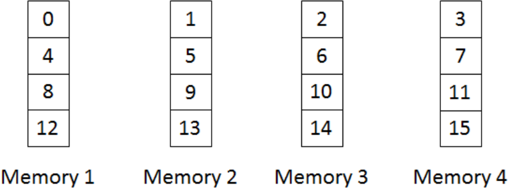
\includegraphics[width=\hsize]{Figures/cyclic_partition_array}
  \caption{Array of 16 elements distributed in a cyclic way on 4 memory
    banks. The numbers represent the indices of the array elements stored
    on the memory banks.}
  \label{fig:cyclic-array}
\end{figure}

\begin{figure}
  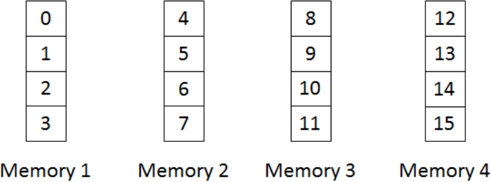
\includegraphics[width=\hsize]{Figures/block_partition_array}
  \caption{Array of 16 elements distributed by blocks on 4 memory
    banks. The numbers represent the indices of the array elements stored
    on the memory banks.}
  \label{fig:block-array}
\end{figure}

\begin{figure}
  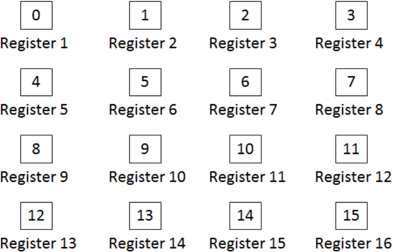
\includegraphics[width=\hsize]{Figures/complete_partition_array}
  \caption{Complete partition of an array of 16 elements, with 1 element
    by register.}
  \label{fig:complete-partition-array}
\end{figure}

For example, an array in a program on an FPGA can be distributed on
different memory banks in a cyclic way (Figure~\ref{fig:cyclic-array}),
partitioned by block (Figure~\ref{fig:block-array}) or fully partitioned
(Figure~\ref{fig:complete-partition-array}) for a maximum bandwidth but at
the cost of a very complex routing.


\subsection{Extending SYCL to express array partitioning}
\label{sec:extend-sycl-expr}

Since in C++ there is a \lstinline|std::array|, we introduced a new
\lstinline|cl::sycl::xilinx::partition_array| similar to
\lstinline|std::array| but taking a new templated class parameter to model
the partition.

For now we support only 1-dimension arrays similar to
\lstinline|std::array| because we are waiting for the ISO C++
standardization committee to define multidimensional arrays
\cite{C++:P0009R5:mdspan} so we can align on the same syntax.

\begin{figure*}
  \balloono{comment}{PartitionCyclicblockTriSYCL}{8}{9}
  \balloono{comment}{PartitionCyclicblockTriSYCL}{12}{13}
  \balloono{comment}{PartitionCyclicblockTriSYCL}{14}{15}
  \balloon{comment}{PartitionCyclicblockTriSYCL}{23}{23}
  \balloon{comment}{PartitionCyclicblockTriSYCL}{26}{26}
  \balloon{comment}{PartitionCyclicblockTriSYCL}{31}{31}
  \balloon{comment}{PartitionCyclicblockTriSYCL}{34}{34}
  \balloon{comment}{PartitionCyclicblockTriSYCL}{42}{42}
  \balloon{comment}{PartitionCyclicblockTriSYCL}{48}{48}
  \balloon{comment}{PartitionCyclicblockTriSYCL}{55}{55}
  \balloon{comment}{PartitionCyclicblockTriSYCL}{58}{58}
  \begin{tabular}{c}
    \begin{lstlisting}[basicstyle=\scriptsize,name=PartitionCyclicblockTriSYCL]
cgh.single_task<class add>([=,
                            d_out = drt::accessor<decltype(a_out)> { a_out },
                            d_in1 = drt::accessor<decltype(a_in1)> { a_in1 },
                            d_in2 = drt::accessor<decltype(a_in2)> { a_in2 }
] {
      // Cyclic Partition for A as matrix multiplication needs row-wise
      // parallel access
      xilinx::partition_array<Type, BLOCK_SIZE,
                              xilinx::partition::cyclic<MAX_DIM>> A;
      // Block Partition for B as matrix multiplication needs column-wise
      // parallel access
      xilinx::partition_array<Type, BLOCK_SIZE,
                              xilinx::partition::block<MAX_DIM>> B;
      xilinx::partition_array<Type, BLOCK_SIZE> C;

      // As A and B Matrix are partitioned with the factor of MAX_DIM, so
      // to get parallel row/column access, input square matrix[DIMXDIM]
      // should be written into local Array in MATRIX[MAX_DIM * MAX_DIM]
      // format

      // Burst read for matrix A
      for (int itr = 0, i = 0, j = 0; itr < DIM * DIM; itr++, j++) {
        xilinx::pipeline([&] {
          if (j == DIM) { j = 0; i++; }
          A[i*MAX_DIM + j] = d_in1[itr];
        });
      }

      // Burst read for matrix B
      for (int itr = 0, i = 0, j = 0; itr < DIM * DIM; itr++, j++) {
        xilinx::pipeline([&] {
          if (j == DIM) { j = 0; i++; }
          B[i * MAX_DIM + j] = d_in2[itr];
        });
      }

      for (int i = 0; i < DIM; i++) {
        // As A and B are partition correctly so loop pipelining is
        // applied at 2nd level loop and which will eventually unroll
        // the lower loop
        for (int j = 0; j < DIM ; j++) {
          xilinx::pipeline([&] {
            int result = 0;
            for (int k = 0; k < MAX_DIM; k++) {
                result += A[i * MAX_DIM +  k] * B[k * MAX_DIM + j];
            }
            C[i*MAX_DIM + j] = result;
          });
        }
      }

      // Burst write from output matrices to global memory
      // Burst write from matrix C
      for (int itr = 0, i = 0, j = 0; itr < DIM * DIM; itr++, j++) {
        xilinx::pipeline([&] {
          if (j == DIM) { j = 0; i++; }
          d_out[itr] = C[i * MAX_DIM + j];
        });
      }

  });
    \end{lstlisting}
  \end{tabular}
  \caption{Example of a matrix multiplication using partitioned
    arrays (orange background) and pipelining (blue background).}
  \label{fig:SYCL-partition-cyclic-block}
\end{figure*}

The example on Figure~\ref{fig:SYCL-partition-cyclic-block} shows how
partitioned arrays are used to speed-up the computation, in combination
with pipelining, by reducing the bank conflicts even if the pipelining
increase the bandwidth of the computation.

\begin{figure}
  \begin{tabular}{c}
    \begin{lstlisting}[basicstyle=\scriptsize,name=PartitionCyclicblockTriSYCL]
xilinx::partition_array<float, 16,
                        xilinx::partition::complete<>> h;
     \end{lstlisting}
  \end{tabular}
  \caption{Complete partition of an array of 16 elements, with 1 element
    by register.}
  \label{fig:SYCL-complete-partition-array}
\end{figure}

In a similar way, a complete partitioning could be used as shown on
Figure~\ref{fig:SYCL-complete-partition-array}.


\subsection{Experiments using partitioned arrays}
\label{sec:experiments-partitioned-arrays}

We made some experiments in the same way as in
\S~\ref{sec:experiments-pipelined-dataflow} with the SYCL code shown on
Figure~\ref{fig:SYCL-partition-cyclic-block} and also with non-single
source HLS C++ or OpenCL C kernels, coming from
\cite{Xilinx:GitHub:SDAccel_Examples}.

\begin{figure}
  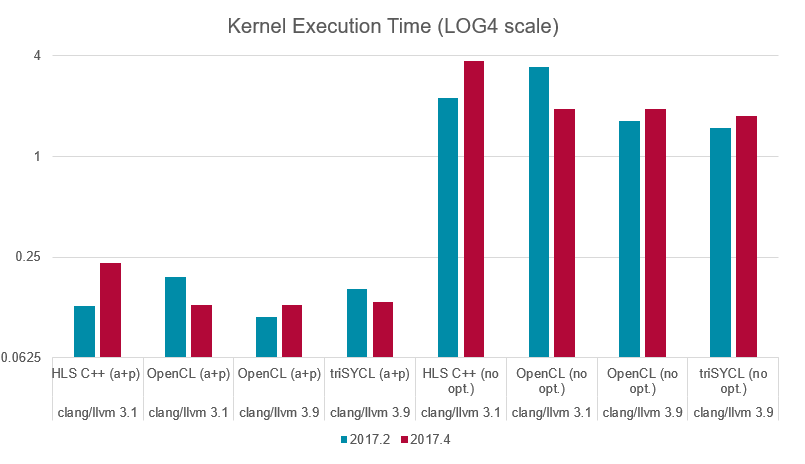
\includegraphics[width=\hsize]{Figures/array_partition_kernel_exe_time}
  \caption{Comparison of execution times of matrix multiplication various
    tools and languages with a Xilinx FPGA acceleration card.}
  \label{fig:matrix-multiplication-benchmark-comparison}
\end{figure}

The performance results are shown on
Figure~\ref{fig:matrix-multiplication-benchmark-comparison} in the same
context as \S~\ref{sec:experiments-pipelined-dataflow}.


The performance of triSYCL are here also quite reasonable compared to some
other programming models and tools, while never reaching the best
performance but for the unoptimized case.


\section{Conclusion}
\label{sec:conclusion}

C++ provides direct mapping to hardware and zero-overhead abstraction, as
summarized by Bjarne Stroustrup in 2 lines. With modern C++, there are
less reasons to choose between ``slow and convenient'' and ``fast and
hard-to-use'' programming models and we are seeing more an evolution from
``fast and hard-to-use'' towards a ``fast and easy-to-use'' paradigm.

At the same time, heterogeneous computing in embedded and high-performance
computing is here to stay because of physical constraints. This puts the
pressure on the programmers to integrate a full system across the various
accelerators. The SYCL standard C++ DSeL allows a single-source approach
for both host and accelerators parts in type-safe way to simplify the
process while interoperable with the ubiquitous C/C++ world. The SYCL
runtime provides an implicit task graph managing asynchronicity and data
transfers across the various memory spaces.

SYCL is one of the candidates inside the ISO C++ committee to push
more heterogeneous computing as a first-class citizen into the
language and is an experimental sand-box to show-case new
non-functional concepts such as the pipelining/dataflow execution
models or the way some arrays are implemented. Our early experiments
with triSYCL show that it has the potential to be competitive with
other more conventional programming tools and languages, even if it is
only done with a research prototype and we have not looked deeply in
the understanding of the current performance results among the
different tools and their versions.

With even more modern meta-programming features comping into C++ such as
introspection and generative programming
\cite{C++:P0194R5:static-reflection,
  C++:P0707R3:metaclasses-generative-C++}, this brings directly at the C++
level some system-wide design capabilities with some software-hardware
trade-offs, without requiring some external generative tools

%\clearpage
% Actually a new column, to avoid an URL in the bibliography to be broken
% across pages triggering the bug
% https://github.com/ho-tex/hyperref/issues/19 mentionned in the
% preamble...
\newpage
\bibliographystyle{ACM-Reference-Format}
\bibliography{biblio}

\end{document}

%%% Local Variables:
%%% mode: latex
%%% TeX-master: t
%%% TeX-auto-untabify: t
%%% TeX-PDF-mode: t
%%% ispell-local-dictionary: "american"
%%% End:
